\documentclass[12pt,a4paper,sans]{moderncv}        % possible options include font size ('10pt', '11pt' and '12pt'), paper size ('a4paper', 'letterpaper', 'a5paper', 'legalpaper', 'executivepaper' and 'landscape') and font family ('sans' and 'roman')

\moderncvstyle{banking}                            % style options are 'casual' (default), 'classic', 'oldstyle' and 'banking'
\moderncvcolor{red}                                % color options 'blue' (default), 'orange', 'green', 'red', 'purple', 'grey' and 'black'
\renewcommand{\familydefault}{\rmdefault}         % to set the default font; use '\sfdefault' for the default sans serif font, '\rmdefault' for the default roman one, or any tex font name
%\nopagenumbers{}                                  % uncomment to suppress automatic page numbering for CVs longer than one page

% character encoding
\usepackage[utf8]{inputenc}                       % if you are not using xelatex ou lualatex, replace by the encoding you are using
%\usepackage{CJKutf8}                              % if you need to use CJK to typeset your resume in Chinese, Japanese or Korean
\usepackage{url}

% adjust the page margins
\usepackage[scale=0.75]{geometry}
%\setlength{\hintscolumnwidth}{3cm}                % if you want to change the width of the column with the dates
%\setlength{\makecvtitlenamewidth}{10cm}           % for the 'classic' style, if you want to force the width allocated to your name and avoid line breaks. be careful though, the length is normally calculated to avoid any overlap with your personal info; use this at your own typographical risks...

% personal data
\name{TheoretiCS Helper\\[.2em]}{for Editors-in-Chief}
%\title{Resumé title}                               % optional, remove / comment the line if not wanted
\address{Nathana\"el Fijalkow, Antoine Amarilli}{}{}% optional, remove / comment the line if not wanted; the "postcode city" and and "country" arguments can be omitted or provided empty
%\phone[mobile]{+33~6~72~51~08~43}                   % optional, remove / comment the line if not wanted
%\phone[fixed]{+2~(345)~678~901}                    % optional, remove / comment the line if not wanted
%\phone[fax]{+3~(456)~789~012}                      % optional, remove / comment the line if not wanted
%\email{nathanael.fijalkow@cs.ox.ac.uk}              % optional, remove / comment the line if not wanted
%\homepage{http://www.liafa.univ-paris-diderot.fr/\textasciitilde nath}                         % optional, remove / comment the line if not wanted
%\extrainfo{additional information}                 % optional, remove / comment the line if not wanted
%\photo[64pt][0.4pt]{picture}                       % optional, remove / comment the line if not wanted; '64pt' is the height the picture must be resized to, 0.4pt is the thickness of the frame around it (put it to 0pt for no frame) and 'picture' is the name of the picture file
%\quote{Some quote}                                 % optional, remove / comment the line if not wanted

\usepackage{amssymb}
\usepackage{amsfonts}
\RequirePackage[language=english,defernumbers=true,style=alphabetic,bibstyle=alphabetic,citestyle=alphabetic,minnames=3,maxnames=99,
maxbibnames=99,sorting=nty,sortcites=false,autopunct=true,backref=false,hyperref=true,backend=bibtex]{biblatex}

\defbibheading{bibempty}{}

\newcommand{\A}{\mathcal{A}}
\newcommand{\B}{\mathcal{B}}
\newcommand{\N}{\mathbb{N}}

\usepackage{framed}

\begin{document}
\makecvtitle

The evaluation of a paper follows a two phase process illustrated in the two flowcharts found in the next two pages.
The flowcharts display the sequence of steps from the paper's point of view.
Solid arrows have a conjuctive semantics: they indicate all necessary next steps. 
On the other hand, dashed arrows are disjunctive: depending on the agent's action, only one arrow is followed.
Texts in red explicit the emails from the Episcience system triggered by the corresponding action.

\vskip1em
TheoretiCS is special in the following aspects:
\begin{itemize}
	\item The first reviewing phase lasts at most 3 months, ensuring to provide quick feedback to the authors with a decision: the paper is either conditionally accepted if the second reviewing phase finds the results to be correct and the presentation of high quality, or rejected.
	\item Both the outcomes of Phase 1 and Phase 2 are collectively decided within the Editorial Board (among editors who declared not having a conflict of interest).
\end{itemize}

\vskip1em
TheoretiCS is an overlay ArXiv journal, meaning that submissions are managed through ArXiv. To submit a paper, the authors first submit to ArXiv, and then to TheoretiCS simply by indicating the ArXiv identifier.
Revisions are also handled through ArXiv: whenever a revised version is requested from the authors, they submit a new version of their paper on ArXiv and report on the revision to TheoretiCS.

\vskip1em



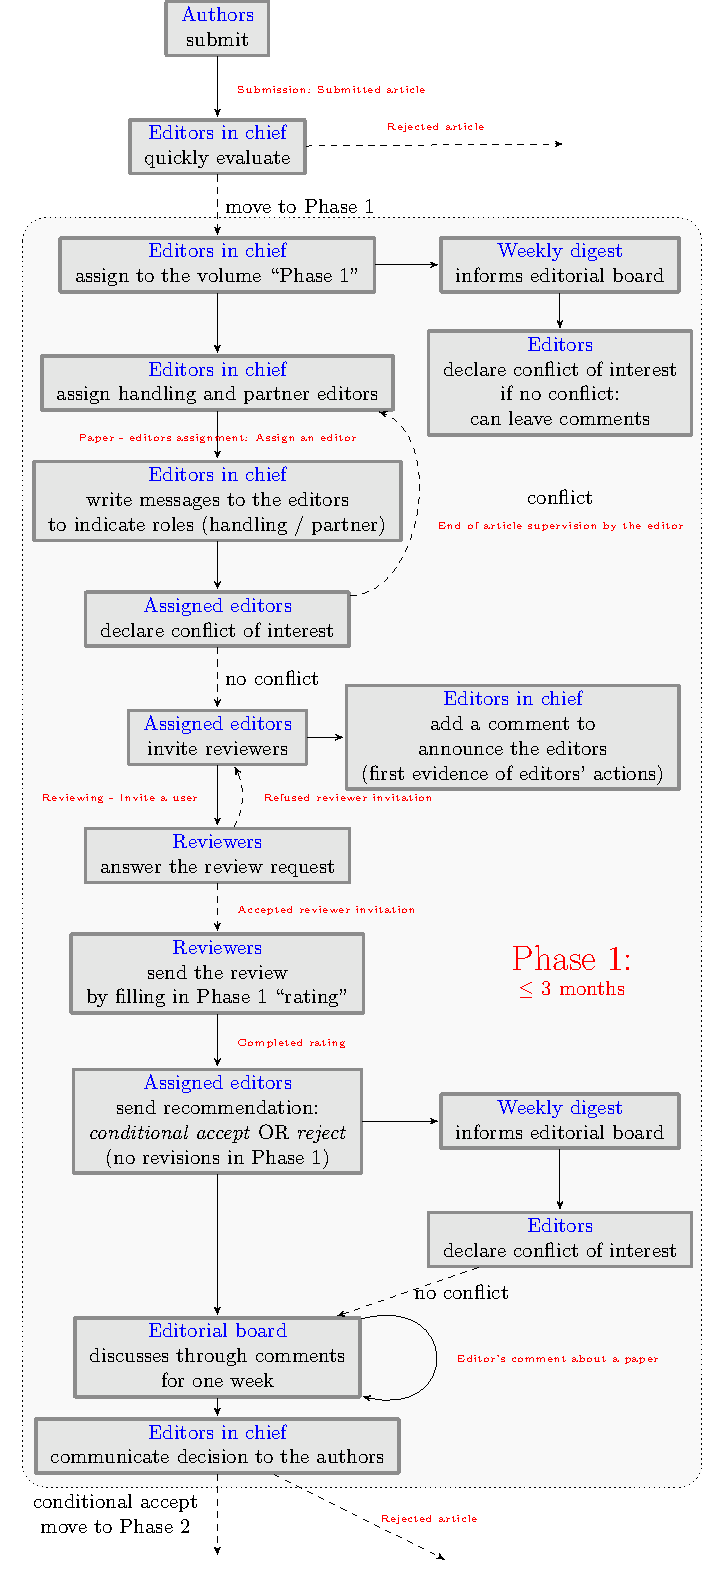
\includegraphics[scale=1]{detailed-phase1}

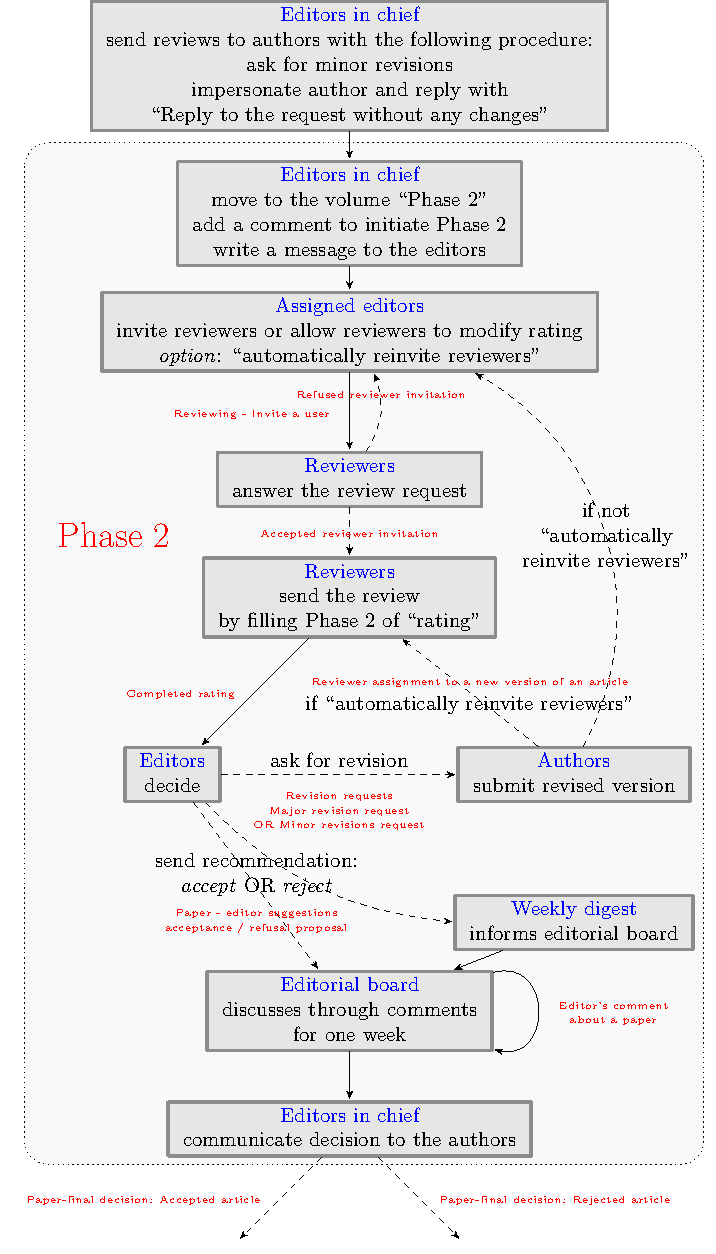
\includegraphics[scale=1]{detailed-phase2}

\end{document}
